\section{Desenvolvimento}
\label{Desenvolvimento}
\subsection{Sinal 1: rampa crescente de 0 a A}:

\begin{figure}[H]
    \centering
    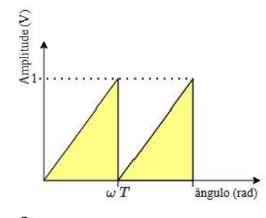
\includegraphics[width=0.6\linewidth]{images/rampa_crescente.png}
    \caption{Sinal de entrada rampa crescente de 0 a P}
    \label{fig:sinal1}
\end{figure}

Para o sinal de entrada rampa crescente de 0 a A, ela pode ser representada por
uma reta que liga o ponto (0,0) ao ponto (P,A). Seu coeficiente angular é dado 
por $\frac{A}{P}$, e a equação da reta é dada por:

\begin{equation}
    v_1(x) = \frac{A}{P}x, 0\leq x < P, v_1(x+P)= v_1(x)
\end{equation}

O valor médio dessa função pode ser calculado pela integral da função em um 
período, dividida pelo período, dessa forma, pode-se calcular esse valor com a 
equação abaixo: 

\begin{equation}
    a_0 = \frac{1}{P} \int_{0}^{P} v_1(x) dx = \frac{1}{P} \int_{0}^{P} \frac{A}{P}x dx = \frac{A}{2}
\end{equation}

Ademais, para construir sua representação em série de Fourier, é necessário 
calcular os coeficientes $a_n$ e $b_n$, que são dados pelas equações abaixo:

\begin{equation}
    \begin{aligned}
        a_n &= \frac{2}{P} \int_{0}^{P} v_1(x)
            \cos\left(\frac{2\pi nx}{P}\right)\,dx \\
            &= \frac{2A}{P^2} \int_{0}^{P} x
            \cos\left(\frac{2\pi nx}{P}\right)\,dx \\
            &= \frac{2A}{P^2} \left[
            \frac{Px}{2\pi n}\sin\left(\frac{2\pi nx}{P}\right)\right. \\
            &\qquad \left.{}+ \frac{P^2}{4\pi^2 n^2}
            \cos\left(\frac{2\pi nx}{P}\right)\right]_{0}^{P} \\
            &= \frac{2A}{P^2} \left[
            \frac{P^2}{4\pi^2 n^2}\cos(2\pi n)
            - \frac{P^2}{4\pi^2 n^2}\cos(0)\right] \\
            &= 0.
    \end{aligned}
\end{equation}
